\begin{frame}[fragile]{Khái niệm Vector nhúng}
\begin{figure}[H]
\centering
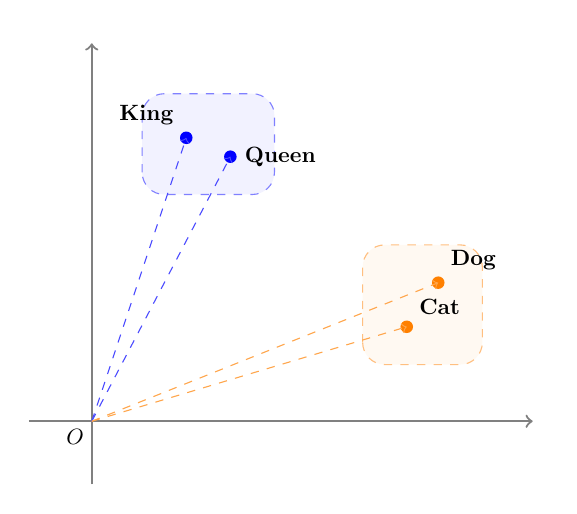
\begin{tikzpicture}[
scale=0.8, % Phóng to toàn bộ tọa độ lên 0.8 lần để vừa slide
every node/.style={scale=0.8}, % Phóng to chữ và node theo tỷ lệ tương ứng
% >=Stealth,
dot/.style={circle, fill=#1, inner sep=2pt},
cluster/.style={dashed, draw=#1!50, fill=#1!5, rounded corners=8pt, inner sep=6pt}
]

% --- Hệ Trục Tọa Độ ---
\draw[->, thick, gray] (-1,0) -- (7,0) node[right, black] {};
\draw[->, thick, gray] (0,-1) -- (0,6) node[above, black] {};
\node[below left] at (0,0) {$O$};

\coordinate (king) at (1.5, 4.5);
\coordinate (queen) at (2.2, 4.2);

\draw[cluster=blue] (0.8, 3.6) rectangle (2.9, 5.2);
\node[blue!80!black, above] at (1.85, 5.2) {};

% Vẽ các điểm và nhãn
\node[dot=blue, label={above left:\textbf{King}}] at (king) {};
\node[dot=blue, label={right:\textbf{Queen}}] at (queen) {};

% Vẽ vector từ gốc tọa độ
\draw[->, blue!70, dashed] (0,0) -- (king);
\draw[->, blue!70, dashed] (0,0) -- (queen);

% --- Cụm 2: Thú cưng (Cat và Dog) ---
\coordinate (cat) at (5.0, 1.5);
\coordinate (dog) at (5.5, 2.2);

% Vùng không gian chung cho cụm Thú cưng
\draw[cluster=orange] (4.3, 0.9) rectangle (6.2, 2.8);
\node[orange!80!black, above] at (5.25, 2.8) {};

% Vẽ các điểm và nhãn
\node[dot=orange, label={above right:\textbf{Cat}}] at (cat) {};
\node[dot=orange, label={above right:\textbf{Dog}}] at (dog) {};

% Vẽ vector từ gốc tọa độ
\draw[->, orange!70, dashed] (0,0) -- (cat);
\draw[->, orange!70, dashed] (0,0) -- (dog);

\end{tikzpicture}
\caption{Ví dụ ánh xạ các vector từ gần nghĩa.}
\end{figure}

\note{
Mô hình ngôn ngữ không đọc chữ trực tiếp mà chia câu thành các phần nhỏ gọi là token và biến chúng thành các vector trong không gian nhiều chiều.
Các từ có ý nghĩa gần nhau như King và Queen, hay Cat và Dog sẽ được ánh xạ vào các vị trí rất gần nhau trong không gian vector này.
Trong đồ án, em sử dụng mô hình vietnamese-sbert của HuggingFace để tạo ra vector nhúng SBERT 768 chiều cho tiếng Việt.
}
\end{frame}
% TODO: thêm logo HuggingFace?
